% Provenance (never printed): old premiere S material on the oceanic lithosphere
% (ophiolite-type layering, peridotite and gabbro, partial melting by decompression
% at the ridge, hydrothermalism, cooling and subsidence of the lithosphere with
% age); see sources/book2/PROVENANCE.md. Melting from figdata/grade-11/
% ridge_melting.py (adiabat and Hirschmann solidus), depth against age from
% depth_age.py (ETOPO1 and the Seton 2020 age grid). Partial melting is re-founded
% in Year 2 (mantle-melting); fault is Book 1's (g7), normal fault is defined here.
\chapter{Las dorsales oceánicas y la litosfera oceánica}\label{ch:g11:ocean-ridges}

En febrero de 1977, un trineo con cámaras remolcado a 2500 metros de
profundidad sobre el rift de las Galápagos, en el Pacífico oriental,
fotografió fotograma tras fotograma la lava negra y desnuda de la dorsal.
Entonces su termómetro registró una pequeña subida de la temperatura del agua,
y en las fotografías la lava aparecía cubierta de cientos de almejas blancas.
Pocos días después, el sumergible \emph{Alvin} llevó a dos geólogos hasta el
lugar: de las grietas de la lava salía agua templada y temblorosa, y a su
alrededor vivían almejas tan largas como un antebrazo, mejillones y cangrejos
blancos; en una inmersión posterior, gusanos de tubo con penachos rojos. Nadie
esperaba encontrar vida allí, así que no había ningún biólogo a bordo. Este
capítulo explica lo que habían encontrado los geólogos: cómo se forma el fondo
oceánico en las dorsales, por qué allí está caliente y qué es de él a medida
que se aleja.
% ledger: whoi:alvin-1977

\begin{recall}
En las dorsales se forma nuevo fondo oceánico, que se aleja hacia ambos lados,
de modo que su edad crece con la distancia al eje; las dorsales forman un
sistema de unos \qty{65000}{km} de longitud, con un valle de rift a lo largo
de las dorsales lentas y una cresta suave a lo largo de las rápidas (el
\cref{ch:g11:drift-to-spreading}). Las placas se separan a ambos lados de una
dorsal a razón de pocos centímetros al año, más deprisa en la dorsal del
Pacífico oriental que en la dorsal mesoatlántica (el \cref{ch:g11:plate-motions}).
La \omterm{def:g11:lithosphere-asthenosphere:lithosphere}{litosfera} es la capa externa rígida, y la \omterm{def:g11:lithosphere-asthenosphere:lithosphere}{astenosfera} que hay debajo fluye;
la temperatura de la \omterm{def:g11:lithosphere-asthenosphere:lithosphere}{astenosfera} solo sube unos \qty{0.45}{\celsius} por
kilómetro de profundidad, y la temperatura de fusión de la roca del manto
aumenta con la profundidad (el \cref{ch:g11:lithosphere-asthenosphere}). El
magma es roca fundida bajo la superficie, el basalto es la roca oscura que
forma la lava al enfriarse, y una falla es una fractura a lo largo de la cual
las rocas se han desplazado (Libro 1, años 6 y 7).
\end{recall}
% ledger: noaa:ridge, katsura10:adiabat, hirschmann:solidus

\section{La litosfera oceánica}

Dos rocas poco frecuentes en la superficie de los continentes forman la mayor
parte de la \omterm{def:g11:ocean-ridges:oceanic-lithosphere}{litosfera oceánica}.

\begin{definition}[Peridotita]\label{def:g11:ocean-ridges:peridotite}
La \emph{peridotita}\index{peridotita} es una roca oscura, de grano grueso,
formada sobre todo por el mineral olivino, con algo de piroxeno. Suele ser
verde y densa. Se cree que gran parte del manto de la Tierra está formada por
peridotita.
\end{definition}

\begin{definition}[Gabro]\label{def:g11:ocean-ridges:gabbro}
El \emph{gabro}\index{gabro} es una roca ígnea oscura, de grano grueso,
formada principalmente por feldespato plagioclasa y piroxeno. Tiene la misma
composición que el basalto, pero cristalizó lentamente, a gran profundidad, lo
que dio tiempo a sus cristales para crecer. Es la roca más abundante de la
\omterm{def:g11:ocean-ridges:oceanic-lithosphere}{corteza oceánica} profunda.
\end{definition}
% ledger: geo:peridotite, geo:gabbro

Los minerales que se nombran aquí, olivino, piroxeno y feldespato, se
describen en el \cref{ch:g11:minerals}.

\begin{omfigure}
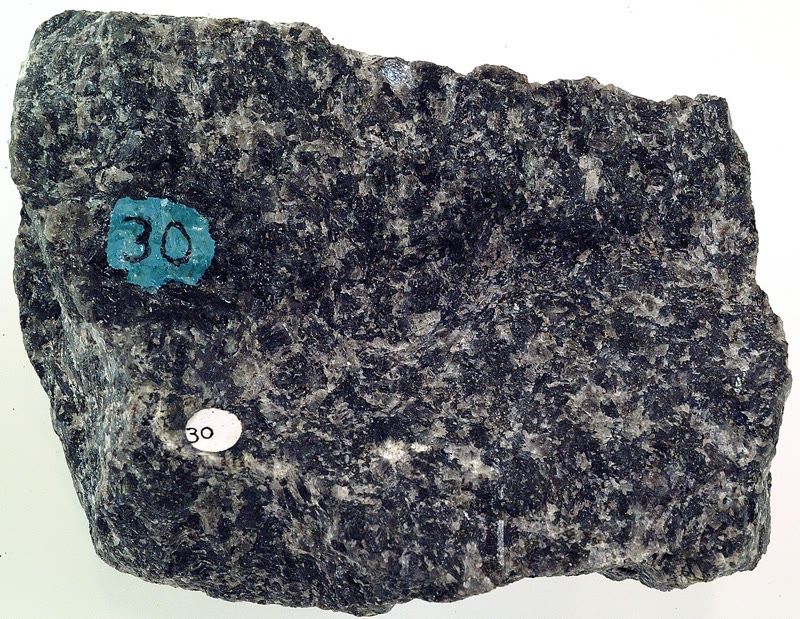
\includegraphics[height=4.2cm]{images/book2/g11-geodil-gabbro.jpg}\hspace{0.03\linewidth}%
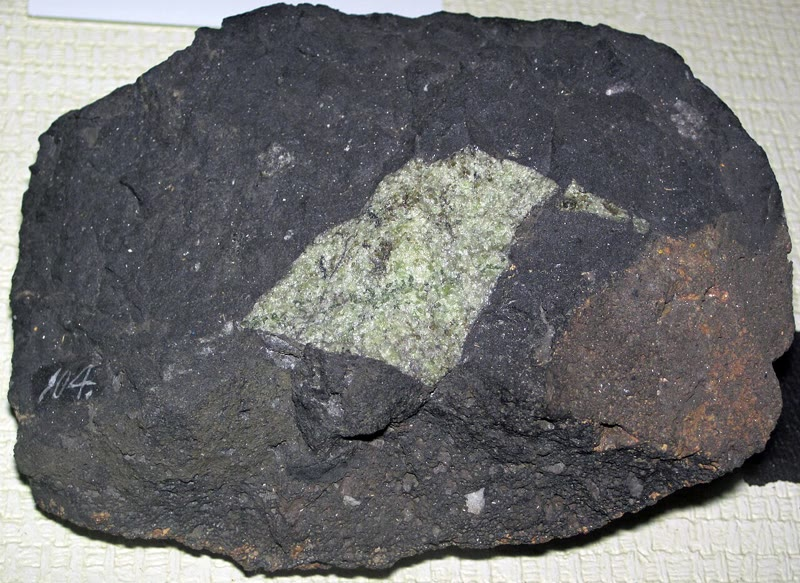
\includegraphics[height=4.2cm]{images/book2/g11-stjohn-peridotite.jpg}

{\small A la izquierda: \omterm{def:g11:ocean-ridges:gabbro}{gabro}, de \qty{9}{cm} de ancho, con cristales de
piroxeno oscuro y de feldespato claro lo bastante grandes para verse;
fotografía de Darla Sondrol (CC0). A la derecha: un trozo de \omterm{def:g11:ocean-ridges:peridotite}{peridotita} verde
del manto, subido dentro de la lava basáltica negra de un volcán de Arizona;
fotografía de James St.~John (CC~BY~2.0).}
\end{omfigure}
% ledger: photo:g11-gabbro, photo:g11-peridotite

\begin{definition}[Corteza oceánica; litosfera oceánica]\label{def:g11:ocean-ridges:oceanic-lithosphere}
La \emph{corteza oceánica}\index{corteza oceanica@corteza oceánica} es la corteza del fondo
oceánico: unos \qty{7}{km} de basalto y \omterm{def:g11:ocean-ridges:gabbro}{gabro}, formados en las dorsales. La
\emph{litosfera oceánica}\index{litosfera oceanica@litosfera oceánica} es la corteza oceánica
junto con la \omterm{def:g11:ocean-ridges:peridotite}{peridotita} rígida de la parte más alta del manto que hay debajo.
\end{definition}

Los estudios sísmicos de todos los océanos dan a la \omterm{def:g11:ocean-ridges:oceanic-lithosphere}{corteza oceánica} un
espesor medio de \qty{7.1}{km}, con un margen de \qty{0.8}{km}, lejos de las
zonas de fractura y de los puntos calientes. Sus capas se conocen gracias a
perforaciones profundas y a láminas de fondo oceánico antiguo empujadas sobre
los continentes. En 2005, un buque de perforación terminó un sondeo de
\qty{1507}{m} de profundidad en una corteza de 15 millones de años del
Pacífico oriental, el primero que pasó de las lavas, a través de los diques,
a los \omterm{def:g11:ocean-ridges:gabbro}{gabros}:
% ledger: white92:crust, iodp1256:section, geo:peridotite

\begin{itemize}
  \item arriba, una delgada cubierta de \emph{sedimentos}, ausente en el eje
        de la dorsal y más gruesa sobre el fondo más antiguo;
  \item más de \qty{800}{m} de \emph{lavas basálticas}, emitidas sobre el
        fondo marino en coladas tabulares y en \emph{almohadillas}, tubos y
        bolas redondeados de lava con una piel vítrea;
  \item el \emph{complejo de diques laminares}, de \qty{346}{m} en este
        sondeo: cientos de láminas verticales de basalto, cada una la grieta
        solidificada por la que el magma subió hacia una erupción, unas junto
        a otras como las páginas de un libro;
  \item el \emph{\omterm{def:g11:ocean-ridges:gabbro}{gabro}}, alcanzado a \qty{1407}{m} bajo el fondo marino, el
        magma que cristalizó lentamente bajo los diques, hasta el \omterm{def:g11:seismic-structure:moho}{Moho};
  \item bajo el \omterm{def:g11:seismic-structure:moho}{Moho}, la \emph{\omterm{def:g11:ocean-ridges:peridotite}{peridotita}} del manto.
\end{itemize}
% ledger: iodp1256:section, geo:basalt-ridges, geo:gabbro

\begin{omfigure}
\begin{tikzpicture}[x=1cm, y=-0.55cm, font=\footnotesize]
% to scale in depth: lavas 0.8 km, dykes 0.35 km (iodp1256:section), crust 7.1 km (white92:crust)
  \fill[omLithAlluv] (0,-0.25) rectangle (2.4,0);
  \fill[lith basalt] (0,0) rectangle (2.4,0.8);
  \fill[omLithBasalt!60] (0,0.8) rectangle (2.4,1.15);
  \foreach \x in {0.15,0.35,...,2.3} \draw[black!55, line width=0.3pt] (\x,0.8) -- (\x,1.15);
  \fill[lith gabbro] (0,1.15) rectangle (2.4,7.1);
  \fill[lith peridotite] (0,7.1) rectangle (2.4,9.0);
  \draw (0,-0.25) rectangle (2.4,9.0);
  \draw[line width=0.9pt] (0,7.1) -- (2.4,7.1);
  \foreach \d in {0,2,4,6,8} {\draw (-0.1,\d) -- (0,\d); \node[anchor=east] at (-0.1,\d) {\d};}
  \node[rotate=90, anchor=south] at (-0.75,4.5) {profundidad bajo el fondo marino (\unit{km})};
  \draw[black!60] (2.4,-0.13) -- (2.7,-1.0) -- (2.85,-1.0);
  \node[anchor=west] at (2.85,-1.0) {sedimentos};
  \draw[black!60] (2.4,0.4) -- (2.7,0.25) -- (2.85,0.25);
  \node[anchor=west] at (2.85,0.25) {lavas: almohadillas y coladas tabulares};
  \draw[black!60] (2.4,0.98) -- (2.7,1.6) -- (2.85,1.6);
  \node[anchor=west] at (2.85,1.6) {complejo de diques laminares};
  \node[anchor=west] at (2.55,4.1) {gabro};
  \node[anchor=west] at (2.55,7.1) {Moho};
  \node[anchor=west] at (2.55,8.05) {peridotita del manto};
  \draw[decorate, decoration={brace, amplitude=5pt}] (7.9,0) -- (7.9,7.1)
    node[midway, right=7pt, align=left] {corteza oceánica\\unos \qty{7}{km}};
\end{tikzpicture}

{\small Las capas de la \omterm{def:g11:ocean-ridges:oceanic-lithosphere}{corteza oceánica}, a escala en profundidad. Los
espesores de las lavas y de los diques son los del sondeo profundo perforado en
el Pacífico oriental; el espesor total es la media de los estudios sísmicos.
La cubierta de sedimentos se hace más gruesa con la edad del fondo.}
\end{omfigure}
% ledger: iodp1256:section, white92:crust

\begin{omfigure}
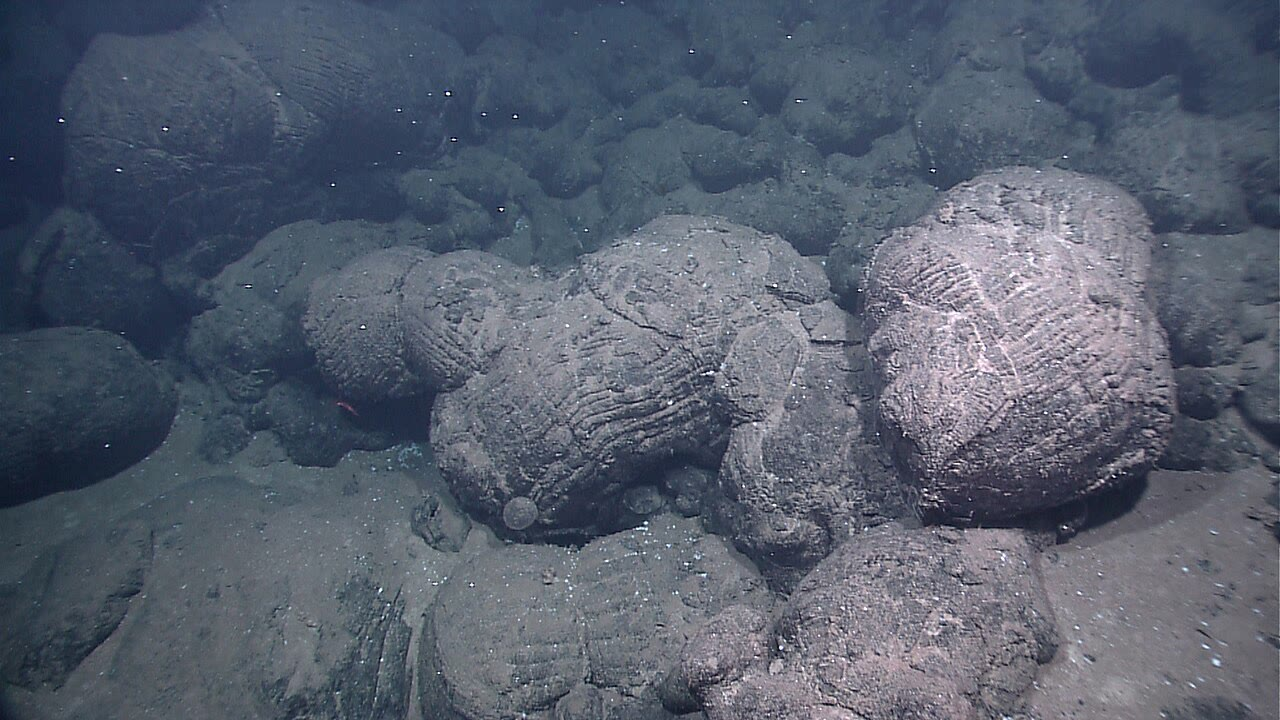
\includegraphics[width=0.8\linewidth]{images/book2/g11-noaa-pillow-lava.jpg}

{\small Lavas almohadilladas en el rift de las Galápagos, a unos 2500 metros
de profundidad, fotografiadas por un vehículo teledirigido en 2011. Cada
almohadilla es una lengua de lava que se solidificó por fuera en cuanto tocó
el agua de mar fría. Fotografía: NOAA Okeanos Explorer Program (dominio
público).}
\end{omfigure}
% ledger: photo:g11-pillow-lava, whoi:alvin-1977 (depth of the rift floor)

\section{Fundirse sin calentarse}

El manto bajo una dorsal es \omterm{def:g11:ocean-ridges:peridotite}{peridotita} sólida, como en todas partes. Sin
embargo, de él salen \qty{7}{km} de basalto y \omterm{def:g11:ocean-ridges:gabbro}{gabro}, una roca fundida que se
ha solidificado. ¿De dónde viene el fundido?

\begin{definition}[Fusión parcial; fusión por descompresión]\label{def:g11:ocean-ridges:partial-melting}
La \emph{fusión parcial}\index{fusion parcial@fusión parcial} es la fusión de solo una parte
de una roca: algunos de sus minerales, o algunos de sus componentes, se
funden, mientras el resto sigue sólido.
La \emph{fusión por descompresión}\index{fusion por descompresion@fusión por descompresión} es la fusión parcial de una roca que asciende, y por tanto está cada
vez menos comprimida, sin que se caliente.
\end{definition}

Cuando dos placas se separan, la \omterm{def:g11:lithosphere-asthenosphere:lithosphere}{astenosfera} asciende bajo la dorsal para
llenar el hueco. Sube demasiado deprisa para perder mucho calor, así que su
temperatura solo baja unos \qty{0.45}{\celsius} por kilómetro durante el
ascenso. Su temperatura de fusión, que depende de la presión, baja mucho más
deprisa: unos \qty{3.9}{\celsius} por kilómetro a \qty{50}{km} de
profundidad. A cierta profundidad, la roca que asciende alcanza su temperatura
de fusión y empieza a fundirse, aunque no se le haya aportado calor.
% ledger: katsura10:adiabat, hirschmann:solidus, white92:crust; computed in
% figdata/grade-11/ridge_melting.py (solidus_slope_50km 3.89)

\begin{method}[¿Dónde se funde el manto que asciende?]\label{met:g11:ocean-ridges:melting}
\begin{enumerate}
  \item Escribe la temperatura de la roca que asciende a cada profundidad: su
        temperatura potencial (la temperatura que tendría en la superficie)
        más \qty{0.45}{\celsius} por kilómetro de profundidad.
  \item Escribe la temperatura de fusión de la roca a cada profundidad, a
        partir de la presión a esa profundidad.
  \item Busca la profundidad a la que las dos son iguales. Más abajo, la roca
        es sólida; más arriba, está parcialmente fundida.
\end{enumerate}
\end{method}

\begin{omfigure}
\begin{tikzpicture}
\begin{axis}[omrecord, omdepth, width=0.72\linewidth, height=6.4cm, xmin=1100, xmax=1700, ymin=0, ymax=150,
  xlabel={temperatura (\unit{\celsius})}, ylabel={profundidad (\unit{km})},
  xticklabel style={/pgf/number format/set thousands separator={}}, clip=true]
% computed in figdata/grade-11/ridge_melting.py; ledger: katsura10:adiabat, hirschmann:solidus, data:prem
\addplot[omProp, line width=1.0pt] table[x=solidus, y=z] {figdata/out/grade-11-ridge_melting-curves.dat};
\addplot[omDef, line width=1.0pt] table[x=ad1300, y=z] {figdata/out/grade-11-ridge_melting-curves.dat};
\addplot[omDef, densely dashed, line width=0.9pt] table[x=ad1400, y=z] {figdata/out/grade-11-ridge_melting-curves.dat};
\addplot[only marks, mark=*, mark size=1.8pt, black] coordinates {(1324.3,54.1) (1438.3,85.0)};
\node[font=\scriptsize, anchor=east, align=right] at (axis cs:1316,62) {la fusión empieza\\a \qty{54}{km}};
\node[font=\scriptsize, anchor=east] at (axis cs:1432,89) {\qty{85}{km}};
\node[font=\scriptsize, text=omProp, anchor=west, align=left] at (axis cs:1560,40) {temperatura\\de fusión};
\node[font=\scriptsize, text=omDef, anchor=east, align=right] at (axis cs:1318,128) {manto que asciende,\\$T_p = \qty{1300}{\celsius}$};
\node[font=\scriptsize, text=omDef, anchor=west, align=left] at (axis cs:1476,140) {$T_p = \qty{1400}{\celsius}$};
\end{axis}
\end{tikzpicture}

{\small La temperatura de la roca del manto que asciende bajo una dorsal (azul)
y su temperatura de fusión (naranja), frente a la profundidad. La roca con una
temperatura potencial de \qty{1300}{\celsius} empieza a fundirse a
\qty{54}{km} de profundidad; la roca \qty{100}{\celsius} más caliente
(discontinua), ya a \qty{85}{km}. Temperatura de fusión de la \omterm{def:g11:ocean-ridges:peridotite}{peridotita} seca
según experimentos (Hirschmann, 2000).}
\end{omfigure}
% values: onset_1300_km 54.1, onset_1400_km 85.0, t_onset_1300 1324 (ridge_melting.py)

\begin{example}[La profundidad de fusión]\label{ex:g11:ocean-ridges:onset}
Para un manto de temperatura potencial \qty{1300}{\celsius}, la roca que
asciende está a $1300 + 0.45 \times 54 \approx \qty{1324}{\celsius}$ cuando
llega a \qty{54}{km}, justo su temperatura de fusión a esa profundidad: la
fusión empieza a unos \qty{54}{km} de profundidad. Por encima, la roca sigue
fundiéndose a medida que asciende.
\end{example}

Solo se funde una pequeña fracción de la \omterm{def:g11:ocean-ridges:peridotite}{peridotita}, y el fundido no es
\omterm{def:g11:ocean-ridges:peridotite}{peridotita}: es basalto. Los fundidos basálticos se reúnen desde toda la región
de fusión, que va desde la profundidad de inicio hasta la base de la corteza;
como son más ligeros que la roca sólida que los rodea, suben hasta el eje de
la dorsal. Allí, parte del magma sale en erupción como lava, parte se
solidifica en forma de diques en las grietas por las que subió, y parte
cristaliza lentamente más abajo como \omterm{def:g11:ocean-ridges:gabbro}{gabro}. La \omterm{def:g11:ocean-ridges:peridotite}{peridotita} sólida que queda,
empobrecida en su basalto, pasa a ser la parte mantélica de la \omterm{def:g11:ocean-ridges:oceanic-lithosphere}{litosfera
oceánica}.
% ledger: asimow01:morb, geo:basalt-ridges, white92:crust

Donde una dorsal cruza una región de manto más caliente, alrededor de un punto
caliente, la fusión empieza a más profundidad, se funde una columna de roca
más larga y se forma más basalto: allí la corteza tiene unos \qty{10}{km} de
espesor en lugar de 7. A la inversa, bajo las dorsales muy lentas el manto que
asciende tiene tiempo de perder calor, se funde menos y forma una corteza
excepcionalmente delgada.
% ledger: white92:crust

\begin{omfigure}
\begin{tikzpicture}[font=\footnotesize]
  % schematic section across a ridge axis, not to scale
  \fill[omSea!45] (-6,0) rectangle (6,1.2);
  \fill[lith basalt] (-6,0) -- (-0.25,0) -- (-0.25,-0.35) -- (-6,-0.6) -- cycle;
  \fill[lith basalt] (6,0) -- (0.25,0) -- (0.25,-0.35) -- (6,-0.6) -- cycle;
  \fill[lith gabbro] (-6,-0.6) -- (-0.25,-0.35) -- (-0.25,-1.4) -- (-6,-1.6) -- cycle;
  \fill[lith gabbro] (6,-0.6) -- (0.25,-0.35) -- (0.25,-1.4) -- (6,-1.6) -- cycle;
  \fill[lith basalt] (-0.3,0) rectangle (0.3,-0.35);
  \fill[lith gabbro] (-0.3,-0.35) rectangle (0.3,-1.45);
  \fill[omProp!70] (-0.8,-0.75) .. controls (-0.4,-0.55) and (0.4,-0.55) .. (0.8,-0.75)
     .. controls (0.4,-0.95) and (-0.4,-0.95) .. (-0.8,-0.75);
  \fill[omProp!70] (-0.12,0) rectangle (0.12,-0.62);
  \fill[lith peridotite] (-6,-1.6) -- (-0.25,-1.4) -- (0.25,-1.4) -- (6,-1.6) -- (6,-5) -- (-6,-5) -- cycle;
  % melting region
  \fill[omProp!35] (-3.2,-1.5) -- (0,-4.0) -- (3.2,-1.5) -- cycle;
  \node[align=center] at (0,-2.95) {región de fusión};
  % isotherms deepening away from the axis
  \draw[omDef!70!black, densely dashed] (-6,-2.6) .. controls (-2.5,-2.0) and (-1,-1.1) .. (0,-1.0) .. controls (1,-1.1) and (2.5,-2.0) .. (6,-2.6);
  \draw[omDef!70!black, densely dashed] (-6,-4.2) .. controls (-3,-3.6) and (-1.2,-2.0) .. (0,-1.9) .. controls (1.2,-2.0) and (3,-3.6) .. (6,-4.2);
  \node[text=omDef!70!black, anchor=west] at (6.05,-2.6) {\qty{800}{\celsius}};
  \node[text=omDef!70!black, anchor=west] at (6.05,-4.2) {\qty{1200}{\celsius}};
  % flow arrows
  \draw[-{Stealth[length=5pt]}, line width=0.9pt] (0,-4.9) -- (0,-4.2);
  \draw[-{Stealth[length=5pt]}, line width=0.9pt] (-1.2,-4.8) .. controls (-1.0,-3.8) and (-2.2,-3.2) .. (-3.6,-3.2);
  \draw[-{Stealth[length=5pt]}, line width=0.9pt] (1.2,-4.8) .. controls (1.0,-3.8) and (2.2,-3.2) .. (3.6,-3.2);
  \draw[-{Stealth[length=5pt]}, line width=1.1pt] (-2,0.6) -- (-4,0.6);
  \draw[-{Stealth[length=5pt]}, line width=1.1pt] (2,0.6) -- (4,0.6);
  \node[anchor=south] at (-3,0.65) {placa};
  \node[anchor=south] at (3,0.65) {placa};
  \node[anchor=west] at (1.0,-0.8) {lente de magma};
  \node[anchor=east] at (-6.05,-0.3) {lavas};
  \node[anchor=east] at (-6.05,-1.1) {gabro};
  \node[anchor=east] at (-6.05,-3.3) {manto};
  \node[anchor=north] at (0,-5.05) {el manto asciende y se funde};
\end{tikzpicture}

{\small Un corte a través del eje de una dorsal (un dibujo, no a escala). El
manto asciende bajo el eje y se funde en parte; el fundido se reúne en una
lente de magma bajo el eje y construye la corteza, que las placas se llevan
hacia ambos lados. Las líneas de igual temperatura (discontinuas) están cerca
de la superficie en el eje y cada vez más hondas al alejarse de él: la
\omterm{def:g11:lithosphere-asthenosphere:lithosphere}{litosfera} se engrosa al enfriarse.}
\end{omfigure}

\section{Dorsales rápidas y dorsales lentas}

Las dorsales se abren a velocidades muy distintas. Según los polos de rotación
del \cref{ch:g11:plate-motions}, la dorsal del Pacífico oriental a \ang{30} S
se abre a \qty{14.6}{cm} al año, y la dorsal mesoatlántica a la misma latitud,
a \qty{3.3}{cm} al año. La forma del eje no es la misma.
% ledger: nnr56:poles (computed in plate_velocities.py: epr30s_speed 145.8, atl30s_speed 32.7)

A lo largo de las dorsales lentas, el eje es un valle de 1 a \qty{2}{km} de
profundidad y de 20 a \qty{30}{km} de anchura. Llega demasiado poco magma al
eje para llenar el hueco de forma continua: la \omterm{def:g11:lithosphere-asthenosphere:lithosphere}{litosfera}, fría y frágil, se
estira y se rompe a lo largo de fallas.

\begin{definition}[Falla normal]\label{def:g11:ocean-ridges:normal-fault}
Una \emph{falla normal}\index{falla normal} es una falla inclinada a lo largo
de la cual el bloque situado sobre el plano de falla ha descendido respecto
del bloque situado debajo. Las fallas normales se forman donde la corteza se
estira.
\end{definition}

El valle de una dorsal lenta es un bloque hundido entre \omterm{def:g11:ocean-ridges:normal-fault}{fallas normales}
enfrentadas; casi todas buzan hacia el eje. Un bloque hundido así entre \omterm{def:g11:ocean-ridges:normal-fault}{fallas
normales} se llama \emph{graben} (o fosa tectónica).
% ledger: buck05:valley, usgs:normal-fault

A lo largo de las dorsales rápidas, el magma llega con la frecuencia
suficiente para llenar el hueco. El eje es un alto suave y poco pronunciado,
sobre una lente de magma situada debajo.
% ledger: buck05:valley, noaa:ridge

\begin{omfigure}
\begin{tikzpicture}[font=\footnotesize, x=0.24cm, y=0.9cm]
  % slow ridge: axial valley between normal faults (not to scale, vertical exaggeration)
  \begin{scope}
    \fill[omSea!45] (-15,-0.7) rectangle (15,1.6);
    \fill[lith basalt] (-15,0.9) -- (-9,0.9) -- (-8.5,0.2) -- (-6,0.2) -- (-5.5,-0.6) -- (5.5,-0.6)
      -- (6,0.2) -- (8.5,0.2) -- (9,0.9) -- (15,0.9) -- (15,-2.2) -- (-15,-2.2) -- cycle;
    \draw[black!70] (-15,0.9) -- (-9,0.9) -- (-8.5,0.2) -- (-6,0.2) -- (-5.5,-0.6) -- (5.5,-0.6)
      -- (6,0.2) -- (8.5,0.2) -- (9,0.9) -- (15,0.9);
    \draw[fault] (-9,0.9) -- (-7.4,-2.2);
    \draw[fault] (-6,0.2) -- (-4.6,-2.2);
    \draw[fault] (9,0.9) -- (7.4,-2.2);
    \draw[fault] (6,0.2) -- (4.6,-2.2);
    % slip arrows on the hanging walls (the axis side of each fault): down along the fault
    \foreach \x/\y/\s in {-7.9/-0.5/1, -5.0/-1.3/1, 7.9/-0.5/-1, 5.0/-1.3/-1} {
      \draw[-{Stealth[length=3pt]}, omProp, line width=0.8pt] (\x+0.9*\s,\y+0.45) -- ++(0.3*\s,-0.6);
    }
    \draw[-{Stealth[length=5pt]}, line width=1pt] (-11,1.25) -- (-14,1.25);
    \draw[-{Stealth[length=5pt]}, line width=1pt] (11,1.25) -- (14,1.25);
    \node at (0,-0.25) {valle axial};
    \node[anchor=north, align=center] at (0,-2.25) {dorsal lenta: un valle\\entre fallas normales};
  \end{scope}
  % fast ridge
  \begin{scope}[xshift=8.2cm]
    \fill[omSea!45] (-15,0) rectangle (15,1.6);
    \fill[lith basalt] (-15,0.3) .. controls (-6,0.4) and (-2,0.9) .. (0,0.95) .. controls (2,0.9) and (6,0.4) .. (15,0.3)
      -- (15,-2.2) -- (-15,-2.2) -- cycle;
    \fill[omProp!75] (-2.5,-0.9) .. controls (-1,-0.7) and (1,-0.7) .. (2.5,-0.9) .. controls (1,-1.1) and (-1,-1.1) .. (-2.5,-0.9);
    \draw[black!70] (-15,0.3) .. controls (-6,0.4) and (-2,0.9) .. (0,0.95) .. controls (2,0.9) and (6,0.4) .. (15,0.3);
    \node[anchor=north] at (0,-1.25) {lente de magma};
    \draw[-{Stealth[length=5pt]}, line width=1pt] (-8,1.25) -- (-14,1.25);
    \draw[-{Stealth[length=5pt]}, line width=1pt] (8,1.25) -- (14,1.25);
    \node at (0,1.3) {alto axial};
    \node[anchor=north, align=center] at (0,-2.25) {dorsal rápida: un alto suave\\sobre una lente de magma};
  \end{scope}
\end{tikzpicture}

{\small Cortes a través de una dorsal lenta y de una dorsal rápida (dibujos, no
a escala; la altura está exagerada). A la izquierda: el valle axial de una
dorsal lenta, de 1 a \qty{2}{km} de profundidad, se ha hundido entre \omterm{def:g11:ocean-ridges:normal-fault}{fallas
normales} que buzan hacia el eje (flechas naranjas: los bloques situados sobre
las fallas se deslizan hacia abajo). A la derecha: una dorsal rápida se eleva
suavemente sobre una lente de magma.}
\end{omfigure}
% ledger: buck05:valley

\begin{example}[Una dorsal lenta y una dorsal rápida]\label{ex:g11:ocean-ridges:rates}
En un millón de años, la dorsal del Pacífico oriental a \ang{30} S forma
$\qty{14.6}{cm/yr} \times 10^6\ \text{años} = \qty{146}{km}$ de nuevo fondo
oceánico, \qty{73}{km} a cada lado; la dorsal mesoatlántica a la misma latitud
forma \qty{33}{km}, \qty{16.5}{km} a cada lado. El sondeo profundo del
Pacífico oriental atravesó una corteza formada a más de \qty{20}{cm} al año,
una de las expansiones más rápidas que se han registrado.
\end{example}
% ledger: nnr56:poles (computed), iodp1256:section

\section{Las fuentes hidrotermales}

La corteza joven del eje está caliente y rota por grietas. El agua de mar se
abre paso en ella.

\begin{definition}[Circulación hidrotermal; fumador negro]\label{def:g11:ocean-ridges:hydrothermal}
La \emph{circulación hidrotermal}\index{circulacion hidrotermal@circulación hidrotermal} es el flujo
de agua de mar que baja por las grietas de la \omterm{def:g11:ocean-ridges:oceanic-lithosphere}{corteza oceánica} caliente, donde
la calienta el magma de debajo y reacciona con la roca, y que vuelve a subir
hasta el fondo marino, donde sale por \emph{fuentes hidrotermales}. Un
\emph{fumador negro}\index{fumador negro} es una fuente de la que brota agua
muy caliente que lleva metales disueltos; al encontrarse con el agua de mar
fría, sulfuros de hierro y otros minerales precipitan formando una nube negra,
y construyen una chimenea alrededor de la fuente.
\end{definition}
% ledger: whoi:vents

El agua de los \omterm{def:g11:ocean-ridges:hydrothermal}{fumadores negros} sale de su chimenea, por lo general, a unos
\qty{350}{\celsius}, y las aguas de las fuentes pueden llegar a
\qty{400}{\celsius}. No hierven, porque sobre ellas pesan dos kilómetros y medio
de agua. Las chimeneas pueden crecer más de \qty{10}{m} de altura. Alrededor
de las fuentes, unas bacterias obtienen su energía del sulfuro de hidrógeno
del agua de la fuente y alimentan a gusanos de tubo, gambas y mejillones: de
eso vivían las almejas del rift de las Galápagos. La mayoría de las fuentes
están a lo largo de las dorsales oceánicas.
% ledger: whoi:vents, whoi:alvin-1977

\begin{omfigure}
\begin{minipage}[c]{0.6\linewidth}\centering
\begin{tikzpicture}[font=\scriptsize, x=0.8cm, y=0.62cm]
  \fill[omSea!45] (0,0) rectangle (10,3);
  \fill[lith basalt] (0,0) rectangle (10,-4);
  \fill[omProp!70] (2,-4.6) .. controls (4,-4.0) and (6,-4.0) .. (8,-4.6) -- (8,-5) -- (2,-5) -- cycle;
  \node at (5,-4.7) {magma};
  \fill[black!75] (4.7,0) -- (4.85,1.6) -- (5.15,1.6) -- (5.3,0) -- cycle;
  \fill[black!45, opacity=0.8] (5,1.7) circle (0.35) (5.2,2.2) circle (0.45) (4.9,2.7) circle (0.4);
  \draw[-{Stealth[length=4pt]}, omDef, line width=0.9pt] (1,0) .. controls (1,-2.5) and (2.5,-3.6) .. (4.2,-3.5);
  \draw[-{Stealth[length=4pt]}, omDef, line width=0.9pt] (9,0) .. controls (9,-2.5) and (7.5,-3.6) .. (5.8,-3.5);
  \draw[-{Stealth[length=4pt]}, omProp, line width=1.1pt] (5,-3.3) -- (5,-0.1);
  \node[align=center, text=omDef!80!black] at (1.6,1.0) {entra agua\\de mar fría};
  \node[align=left, anchor=west] at (5.6,1.4) {fumador negro,\\unos \qty{350}{\celsius}};
  \node[align=left, anchor=west, text=omProp!80!black, fill=white, fill opacity=0.85, text opacity=1, inner sep=1.5pt] at (5.3,-1.8) {se calienta\\y sube};
\end{tikzpicture}
\end{minipage}\hfill
\begin{minipage}[c]{0.3\linewidth}\centering
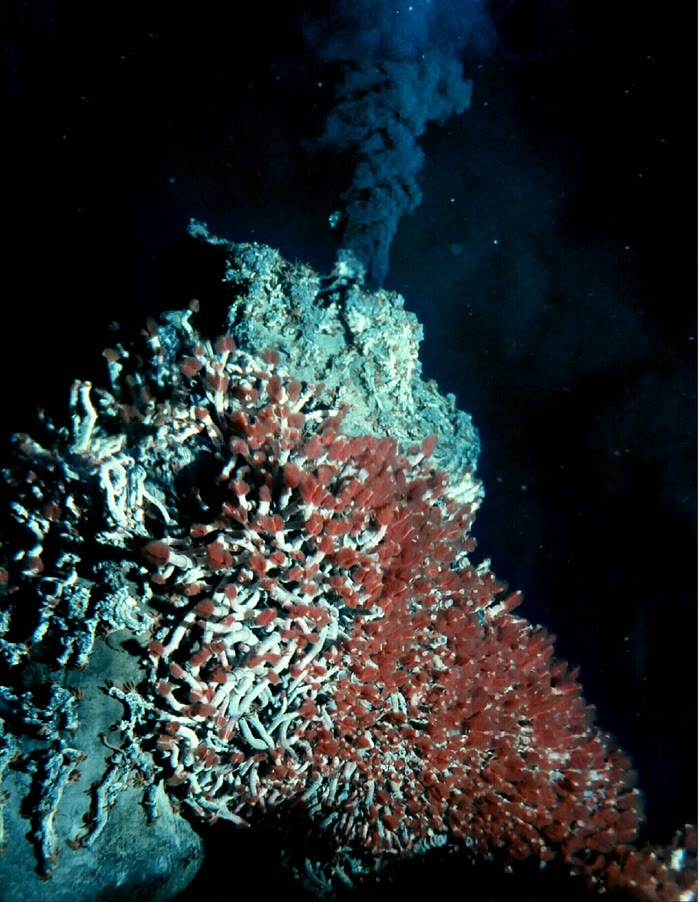
\includegraphics[width=\linewidth]{images/book2/g11-noaa-black-smoker.jpg}
\end{minipage}

{\small A la izquierda: \omterm{def:g11:ocean-ridges:hydrothermal}{circulación hidrotermal} en el eje de una dorsal (un
dibujo, no a escala). A la derecha: un \omterm{def:g11:ocean-ridges:hydrothermal}{fumador negro} en la dorsal de Juan de
Fuca, con la chimenea cubierta de gusanos de tubo de branquias rojas;
fotografía de la Universidad de Washington y la NOAA (dominio público).}
\end{omfigure}
% ledger: whoi:vents, photo:g11-black-smoker

\begin{history}[El \emph{Alvin} en el rift de las Galápagos, 1977]
La expedición, financiada por la National Science Foundation, empezó el
8~de febrero de 1977 a bordo del buque oceanográfico \emph{Knorr}. El trineo
con cámaras ANGUS, remolcado a \qty{2500}{m} de profundidad sobre el rift,
registró una subida de la temperatura del agua, y en los mismos fotogramas
sus fotografías mostraron cientos de almejas blancas y conchas pardas de
mejillón sobre la lava. En la inmersión 713 del \emph{Alvin}, los geólogos
Jack Corliss y Tjeerd van Andel encontraron agua a \qty{8}{\celsius} que
salía temblorosa de las grietas, y luego hasta a \qty{17}{\celsius}, mientras
que el agua profunda de alrededor estaba a \qty{2}{\celsius}; almejas blancas
de hasta \qty{30}{cm} de largo cubrían una zona de unos \qty{50}{m} de ancho.
No había ningún biólogo a bordo: la expedición había ido a buscar el agua
caliente, y encontró una comunidad de animales que nadie había imaginado.
\end{history}
% ledger: whoi:alvin-1977

\section{Enfriarse, engrosarse, hundirse}

Al alejarse del eje, la \omterm{def:g11:lithosphere-asthenosphere:lithosphere}{litosfera} se enfría desde arriba, a través del océano
frío que tiene encima. La capa enfriada se hace más gruesa con el tiempo: la
\omterm{def:g11:lithosphere-asthenosphere:lithosphere}{litosfera} se engrosa, desde pocos kilómetros en el eje hasta unos cien
kilómetros bajo el fondo antiguo. La roca enfriada se contrae y se vuelve más
densa, así que la \omterm{def:g11:lithosphere-asthenosphere:lithosphere}{litosfera} flota más baja sobre la \omterm{def:g11:lithosphere-asthenosphere:lithosphere}{astenosfera} (\omterm{def:g11:lithosphere-asthenosphere:isostasy}{isostasia}, el
\cref{ch:g11:lithosphere-asthenosphere}): el fondo oceánico se hunde a medida
que envejece. En un cuerpo que se enfría por conducción desde su superficie,
el espesor de la capa enfriada crece como la raíz cuadrada del tiempo.
% ledger: ps77:depth-age, rs09:lab

\begin{proposition}[Profundidad del fondo oceánico frente a su edad]\label{prop:g11:ocean-ridges:depth-age}
De media, el fondo oceánico de edad $t$ (en millones de años) está a la
profundidad
\[
  d(t) = 2500 + 350\sqrt{t} \quad \text{metros} \qquad (0 \le t \le 70),
\]
y, para el fondo de más de unos 20 millones de años,
\[
  d(t) = 6400 - 3200\,e^{-t/62.8} \quad \text{metros}:
\]
el fondo se hunde deprisa mientras es joven, y luego cada vez más despacio,
hacia unos \qty{6400}{m}. (Se admite: Parsons y Sclater ajustaron en 1977 las
fórmulas a las profundidades del Pacífico norte y del Atlántico norte,
corregidas del peso de sus sedimentos.)
\end{proposition}
% ledger: ps77:depth-age

La raíz cuadrada hace que el fondo joven se hunda deprisa: en su primer millón
de años el fondo se hunde \qty{350}{m}, en los tres millones de años
siguientes otros \qty{350}{m}, y entre 16 y 64 millones de años \qty{1400}{m},
tanto como en sus primeros dieciséis millones de años. La ley exponencial
describe cómo deja de hundirse el fondo antiguo: se comporta como si la placa
que se enfría tuviera un espesor fijo, de unos \qty{125}{km}.
% ledger: ps77:depth-age

\begin{omfigure}
\begin{tikzpicture}
\begin{axis}[omrecord, omdepth, width=0.82\linewidth, height=6.2cm, xmin=0, xmax=180, ymin=2000, ymax=6600,
  xlabel={edad del fondo oceánico (millones de años)}, ylabel={profundidad (\unit{m})},
  yticklabel style={/pgf/number format/set thousands separator={}},
  legend style={font=\scriptsize, at={(0.5,-0.32)}, anchor=north, legend columns=3, /tikz/every even column/.append style={column sep=6pt}}, legend cell align=left]
% computed in figdata/grade-11/depth_age.py; ledger: data:etopo1, data:b2-seafloor-age, ps77:depth-age
\addplot[only marks, mark=*, mark size=1.3pt, black!70, error bars/.cd, y dir=both, y explicit]
  table[x=age, y=depth, y error minus=em, y error plus=ep] {figdata/out/grade-11-depth_age-bins.dat};
\addplot[omProp, line width=1.0pt] table[x=age, y=depth] {figdata/out/grade-11-depth_age-sqrt.dat};
\addplot[omDef, line width=1.0pt, densely dashed] table[x=age, y=depth] {figdata/out/grade-11-depth_age-exp.dat};
\legend{{medido: mediana y mitad central}, {$2500 + 350\sqrt{t}$}, {$6400 - 3200\,e^{-t/62.8}$}}
\end{axis}
\end{tikzpicture}

{\small Profundidad del fondo oceánico frente a su edad: para cada franja de
edad de 5 millones de años, la profundidad mediana de todas las celdas de un
grado de los océanos del mundo, y el intervalo que ocupa la mitad central de
ellas. El fondo joven sigue de cerca la ley de la raíz cuadrada; el fondo más
antiguo queda menos hondo que las leyes, porque sus celdas incluyen
sedimentos y volcanes. Datos: ETOPO1 (NOAA) y las edades del fondo oceánico
de Seton y colaboradores (2020); leyes de Parsons y Sclater (1977).}
\end{omfigure}
% values (depth_age.py): median 2.5-5 Myr 3114 (law 3178), 60-65 Myr 4648 (law 5267), fit a 2727 b 255

Las profundidades medidas del fondo joven concuerdan con la ley con un margen
de unos \qty{100}{m}. En el fondo más antiguo, las medianas medidas quedan
varios cientos de metros por encima de las leyes. Las leyes describen la
profundidad del propio fondo, como si se quitaran sus sedimentos; las celdas
medidas conservan sus sedimentos, que se hacen más gruesos con la edad del
fondo y superan el kilómetro de espesor en el fondo más antiguo del oeste del
Atlántico norte, e incluyen montes submarinos y mesetas volcánicas.
% ledger: ps77:depth-age; values from depth_age.py

La \omterm{def:g11:ocean-ridges:oceanic-lithosphere}{litosfera oceánica} antigua es, por tanto, gruesa, fría y densa. El
capítulo siguiente muestra que puede llegar a ser más densa que la \omterm{def:g11:lithosphere-asthenosphere:lithosphere}{astenosfera}
que tiene debajo, y volver a hundirse en el manto (el \cref{ch:g11:subduction-zones}).

\section{Ejercicios}

\begin{exercise}[$\star$]\label{exo:g11:ocean-ridges:1}
Define la \omterm{def:g11:ocean-ridges:peridotite}{peridotita} y el \omterm{def:g11:ocean-ridges:gabbro}{gabro}. ¿Cuál de los dos pertenece a la \omterm{def:g11:ocean-ridges:oceanic-lithosphere}{corteza
oceánica}, y cuál al manto? El \omterm{def:g11:ocean-ridges:gabbro}{gabro} tiene la misma composición que el
basalto: ¿por qué sus cristales son mucho más grandes?
\end{exercise}

\begin{exercise}[$\star$]\label{exo:g11:ocean-ridges:2}
Enumera las capas de la \omterm{def:g11:ocean-ridges:oceanic-lithosphere}{litosfera oceánica} desde el fondo marino hacia abajo.
El sondeo profundo del Pacífico oriental llegó a \qty{1507}{m} bajo el fondo
marino: ¿qué fracción de una corteza de \qty{7.1}{km} atravesó?
\end{exercise}

\begin{exercise}[$\star$]\label{exo:g11:ocean-ridges:3}
Con $d = 2500 + 350\sqrt{t}$, halla la profundidad de un fondo oceánico de 0,
9 y 25 millones de años.
\end{exercise}

\begin{exercise}[$\star$]\label{exo:g11:ocean-ridges:4}
Define una \omterm{def:g11:ocean-ridges:normal-fault}{falla normal}. En una dorsal lenta, ¿qué fuerza forma las \omterm{def:g11:ocean-ridges:normal-fault}{fallas
normales}, y en qué sentido se mueven los bloques situados sobre las fallas?
\end{exercise}

\begin{exercise}[$\star$]\label{exo:g11:ocean-ridges:5}
El agua de los \omterm{def:g11:ocean-ridges:hydrothermal}{fumadores negros} sale a unos \qty{350}{\celsius}. ¿Por qué no
hierve? ¿Qué es el ``humo'' negro?
\end{exercise}

\begin{exercise}[$\star\star$]\label{exo:g11:ocean-ridges:6}
Con la figura de la fusión: (1) ¿a qué profundidad empieza a fundirse un manto
de temperatura potencial \qty{1300}{\celsius}, y a qué temperatura? (2) ¿Y un
manto \qty{100}{\celsius} más caliente? (3) ¿Cuál de los dos forma la corteza
más gruesa? ¿Por qué?
\end{exercise}

\begin{exercise}[$\star\star$]\label{exo:g11:ocean-ridges:7}
La roca del manto que asciende, de temperatura potencial \qty{1300}{\celsius},
está a \qty{1345}{\celsius} a \qty{100}{km} de profundidad, donde su
temperatura de fusión es de \qty{1489}{\celsius}. (1) ¿Cuántos grados le faltan
para su temperatura de fusión? (2) Empieza a fundirse a \qty{54}{km}. ¿En
cuántos grados por kilómetro, de media, se ha cerrado la diferencia durante el
ascenso? (3) ¿Se ha calentado la roca?
\end{exercise}

\begin{exercise}[$\star\star$]\label{exo:g11:ocean-ridges:8}
La dorsal del Pacífico oriental se abre a \qty{14.6}{cm} al año a \ang{30} S,
y la dorsal mesoatlántica a \qty{3.3}{cm} al año. Suponiendo una expansión
simétrica, ¿cuánto tarda cada dorsal en formar \qty{1000}{km} de fondo a un
lado?
\end{exercise}

\begin{exercise}[$\star\star$]\label{exo:g11:ocean-ridges:9}
Las dorsales miden unos \qty{65000}{km} de longitud. Supón que se abren de
media a \qty{5}{cm} al año y forman una corteza de \qty{7.1}{km} de espesor.
(1) ¿Qué superficie de nuevo fondo oceánico forman cada año? (2) ¿Qué volumen
de corteza? (3) ¿Cuánto tardarían en formar una superficie igual a la de los
océanos, \qty{3.6e8}{km^2}?
\end{exercise}

\begin{exercise}[$\star\star$]\label{exo:g11:ocean-ridges:10}
Un valle axial tiene \qty{1.5}{km} de profundidad. Se hundió a lo largo de dos
\omterm{def:g11:ocean-ridges:normal-fault}{fallas normales} enfrentadas, cada una con un buzamiento de \ang{60}. (1) ¿Cuánto
se desplazó cada falla a lo largo de su plano? (2) ¿Cuánto se separaron
horizontalmente los dos lados a causa de las dos fallas? (3) El valle tiene
\qty{25}{km} de anchura: ¿lo formó solo el fallamiento?
\end{exercise}

\begin{exercise}[$\star\star$]\label{exo:g11:ocean-ridges:11}
Con $d = 6400 - 3200\,e^{-t/62.8}$, halla la profundidad de un fondo de 25 y
100 millones de años, y cuánto se hunde el fondo entre esas edades. Compara el
primer valor con el de la ley de la raíz cuadrada.
\end{exercise}

\begin{exercise}[$\star\star\star$]\label{exo:g11:ocean-ridges:12}
Una columna de manto de \qty{100}{km} de espesor se enfría de media
\qty{700}{\celsius}. La roca se contrae $\alpha = 3.2 \times 10^{-5}$ de su
longitud por cada grado de enfriamiento. (1) ¿Cuánto se acorta la columna?
(2) Al hundirse, el agua de mar (\qty{1025}{kg/m^3}) llena el espacio que
queda encima; con una densidad del manto de \qty{3380}{kg/m^3}, la \omterm{def:g11:lithosphere-asthenosphere:isostasy}{isostasia}
hace que el fondo se hunda
$s = \rho_m\,\alpha\,\Delta T\,L/(\rho_m - \rho_w)$. Calcula $s$. (3) Compara
con el hundimiento total que permite la ley exponencial, de \qty{2500}{m} a
\qty{6400}{m}.
\end{exercise}

\begin{exercise}[$\star\star\star$]\label{exo:g11:ocean-ridges:13}
La fusión empieza a \qty{54}{km} de profundidad en un manto a
\qty{1300}{\celsius}, y a \qty{85}{km} en uno a \qty{1400}{\celsius}; en los
dos, la fusión continúa hasta la base de la corteza, a unos \qty{7}{km} de
profundidad. (1) Compara las longitudes de las dos columnas de fusión. (2) Si
cada kilómetro de roca que asciende diera la misma cantidad de fundido, ¿qué
espesor tendría la corteza sobre el manto más caliente, para una corteza de
\qty{7.1}{km} sobre el manto normal? (3) Compáralo con los \qty{10.3}{km}
medidos donde las dorsales encuentran un manto más caliente.
\end{exercise}

\begin{exercise}[$\star\star\star$]\label{exo:g11:ocean-ridges:14}
Las profundidades medianas medidas del fondo oceánico son \qty{3114}{m} a una
edad de \num{3.75} millones de años, \qty{4018}{m} a \num{22.5}, \qty{4465}{m}
a \num{42.5} y \qty{4648}{m} a \num{62.5}. (1) Calcula la profundidad que da
la ley de la raíz cuadrada a cada edad, y la diferencia con la medida. (2)
¿Cómo cambia la diferencia con la edad? (3) Explícalo.
\end{exercise}

\begin{exercise}[$\star\star\star$]\label{exo:g11:ocean-ridges:15}
El punto crítico del agua está a \qty{374}{\celsius} y \qty{22.064}{MPa}: por
encima de esa presión, el agua no hierve a ninguna temperatura. (1) Calcula la
presión del agua a \qty{2500}{m} de profundidad (agua de mar a
\qty{1025}{kg/m^3}, $g = \qty{9.8}{m/s^2}$, más los \qty{0.1}{MPa} de la
atmósfera). (2) ¿Puede hervir el agua de una fuente a esa profundidad, por
caliente que esté? (3) ¿Por debajo de qué profundidad, aproximadamente, se
cumple esto para todas las fuentes?
\end{exercise}

\section{Problema: la vida de un trozo de fondo del Pacífico}

\begin{problem}[{Problema de fin de semana --- de la dorsal al océano profundo}]
\label{pb:g11:ocean-ridges:1}
% values: EPR 30 S full rate 145.8 mm/yr (plate_velocities.py, nnr56:poles); depth law
% ps77:depth-age; crust white92:crust; alpha ps77; densities data:prem; median 60-65 Myr
% 4648 m (depth_age.py)
Un trozo de fondo oceánico nace hoy en la dorsal del Pacífico oriental a
\ang{30} S, donde las placas del Pacífico y de Nazca se separan a
\qty{14.6}{cm} al año. Se desplaza hacia el oeste con la placa del Pacífico.
Toma la expansión como simétrica, la corteza de \qty{7.1}{km} de espesor y la
ley de profundidad $d = 2500 + 350\sqrt{t}$ metros ($t$ en millones de años).

\medskip
\noindent\textbf{Parte I --- El nacimiento en la dorsal.}
\begin{enumerate}
  \item ¿Cuál es la semivelocidad de expansión, en centímetros al año y en
        kilómetros por millón de años?
  \item ¿A qué profundidad nace el trozo de fondo?
  \item Enumera las rocas que lo forman, desde el fondo marino hasta la base
        de la \omterm{def:g11:lithosphere-asthenosphere:lithosphere}{litosfera}.
  \item El magma que lo formó procedía del manto de debajo. Explica cómo se
        fundió el manto sin calentarse.
  \item ¿Qué volumen de corteza forma esta dorsal cada millón de años, a
        ambos lados, por cada kilómetro de su longitud?
\end{enumerate}

\medskip
\noindent\textbf{Parte II --- El viaje.}
\begin{enumerate}[resume]
  \item ¿A qué distancia de la dorsal estará el trozo al cabo de 1, 4, 16 y 64
        millones de años, si la velocidad no cambia?
  \item ¿Cuánto tardará en recorrer \qty{2000}{km}?
  \item ¿Por qué la distancia real al cabo de 64 millones de años puede
        diferir de la respuesta de la pregunta~6?
  \item Cerca de la dorsal, el agua de mar circula por la corteza joven y
        sale por fuentes. ¿Por qué se detiene esta circulación en el fondo antiguo?
  \item ¿Sobre qué placa viaja el trozo, y hacia qué tipo de límite de placas
        lo lleva esa placa, por su lado occidental?
\end{enumerate}

\medskip
\noindent\textbf{Parte III --- Hundirse al envejecer.}
\begin{enumerate}[resume]
  \item Calcula su profundidad a 1, 4, 16 y 64 millones de años.
  \item ¿Cuánto se hunde durante sus primeros 16 millones de años, y entre 16
        y 64 millones de años? Coméntalo.
  \item ¿A qué edad llega a una profundidad de \qty{4000}{m}?
  \item Compara su profundidad a 64 millones de años con la ley exponencial,
        $6400 - 3200\,e^{-t/62.8}$.
  \item La profundidad mediana medida del fondo oceánico de 60 a 65 millones
        de años es de \qty{4648}{m}. Explica la diferencia.
\end{enumerate}

\medskip
\noindent\textbf{Parte IV --- Su densidad y su destino.}
\begin{enumerate}[resume]
  \item A los 64 millones de años, toma su \omterm{def:g11:lithosphere-asthenosphere:lithosphere}{litosfera} de \qty{100}{km} de
        espesor y, de media, \qty{700}{\celsius} más fría que la \omterm{def:g11:lithosphere-asthenosphere:lithosphere}{astenosfera}.
        Con $\alpha = 3.2 \times 10^{-5}$ por grado, ¿en qué fracción se ha
        vuelto más densa la parte mantélica? Partiendo de \qty{3380}{kg/m^3},
        ¿cuál es su densidad?
  \item Su corteza tiene \qty{7.1}{km} de espesor, con una densidad de
        \qty{2900}{kg/m^3}. Calcula la densidad media de los
        \qty{100}{km} enteros de \omterm{def:g11:lithosphere-asthenosphere:lithosphere}{litosfera}.
  \item Compárala con la de la \omterm{def:g11:lithosphere-asthenosphere:lithosphere}{astenosfera} que tiene debajo, tomada como
        \qty{3380}{kg/m^3}.
  \item ¿Qué puede hacer una \omterm{def:g11:lithosphere-asthenosphere:lithosphere}{litosfera} así cuando llega a una fosa?
  \item Concluye: ¿a qué profundidad está este trozo de fondo cuando tiene 64
        millones de años?
\end{enumerate}
\end{problem}
